\documentclass[../proyecto.tex]{memoir}

\begin{document}

\chapter{Análisis}

Las estimaciones de los métodos Monte Carlo dependen en gran medida de la anchura del intervalo de confianza $[\mu+3\sigma, \mu-3\sigma]$. Dicha anchura se reduce con el incremento del número de muestras aleatorias pero lo hace lentamente con el consecuente incremento de tiempo de computación. Por esta razón se crean métodos alternativos conocidos como métodos de reducción de la varianza. En esta sección introducimos uno que se adecúa a nuestro problema y que utilizaremos en las todas las ejecuciones posteriores.

\section{Reducción de la varianza}

En la \autoref{fig:3-1} visualizamos la evolución del área del cuadrado más pequeño que contiene a todas las células en cada iteración de juego de vida. Para el contenido de esta sección no es relevante la configuración inicial de la que se han obtenido los datos. Cada punto representa una estimación Monte Carlo, para los puntos de color naranja no se puede rechazar la hipótesis nula de que sigan un distribución normal, los de color azul sí rechazan la hipótesis nula y por tanto no podemos afirmar nada acerca de su intervalo de confianza.

El intervalo de confianza $[\mu+3\sigma, \mu-3\sigma]$ crece a medida que la iteración se aleja de la configuración inicial, de decir, la varianza aumenta. Es posible reducirla aumentando el número de simulaciones globalmente e incrementando notablemente el tiempo de cálculo. Sin embargo para el número prefijado de simulaciones se obtienen intervalos de confianza lo suficientemente pequeños en las iteraciones iniciales, por tanto proponemos incrementar el número de simulaciones a medida que las iteraciones aumenten. Este incremento requiere de la adición de nuevas simulaciones en cada iteración, las cuales serán escogidas aleatoriamente de las ya existentes modificando la semilla para no obtener simulaciones duplicadas. Experimentalmente hemos observado que un valor que muestra buenos resultados sin aumentar excesivamente el tiempo de cálculo es un incremento en cada iteración de una décima parte del valor inicial de simulaciones. Finalmente es posible observar la reducción del intervalo de confianza que conlleva dicho incremento en la \autoref{fig:3-2}.

\begin{figure}[H]
	\centering
    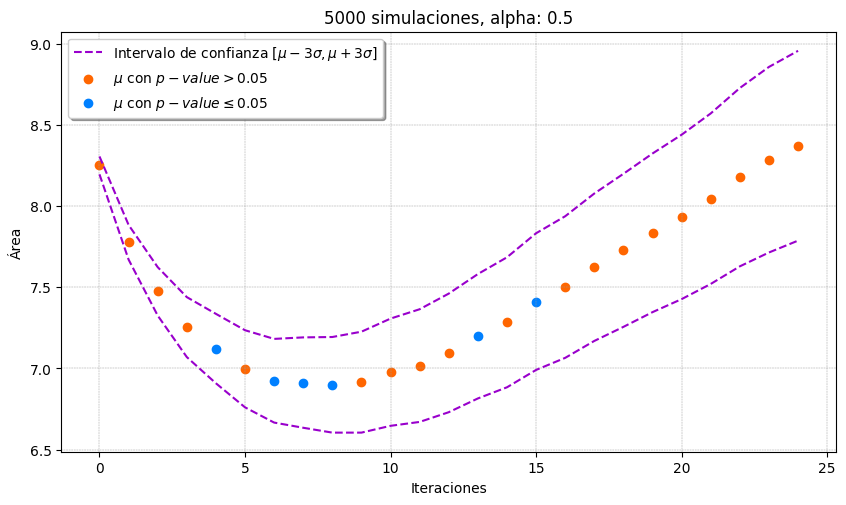
\includegraphics[width=\textwidth]{./images/iteracion_without_inc.png}
    \caption{Ejecución sin incremento del valor inicial de simulaciones cada iteración.}
    \label{fig:3-1}
\end{figure}

\begin{figure}[H]
        \centering
        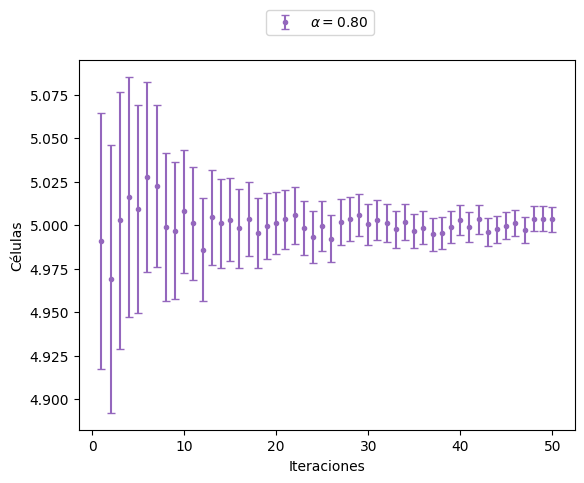
\includegraphics[width=\textwidth]{./images/iteracion_inc.png}
        \caption{Ejecución con incremento del 10\% del valor inicial de simulaciones en cada iteración.}
        \label{fig:3-2}
\end{figure} 

\section{Efecto del $\alpha$-asincronismo en las configuraciones iniciales}

El impacto de la $\alpha$-asíncronicidad se estudiado a través de la ejecución para cada configuración inicial seleccionada en la sección \ref{seleccion} de 50 pasos o iteraciones con los valores de $\alpha$: 0.15, 0.3, 0.45, 0.6, 0.75 y 0.9, y cada iteración simulada 5000 veces aplicando el método de reducción de la varianza de la sección anterior. Como resultado hemos obtenido los valores medios de las variables expuestas en la sección \ref{vars} junto con sus correspondientes intervalos de confianza para cada iteración.

Comentamos los efectos de la variación de la $\alpha$-asincronicidad sobre la configuración inicial \textit{blinker}. Como se observa en las \autoref{fig:blinker1}, \autoref{fig:blinker2} y \autoref{fig:blinker3}, cuando no existe perturbación en el intercambio de información entre células, el calor en cada iteración es 4, es decir, 2 células mueren y 2 células nacen por iteración, ocupa un área de 3 \textit{células}$^2$ y está conformada por un solo clúster. Intuitivamente se puede pensar que valores pequeños de $\alpha$ disminuyen el calor, esto es, la tasa de cambio se hace pequeña y en consecuencia no debería de variar mucho el área que ocupe el patrón, pero por el contrario mientras que efectivamente el calor disminuye, el área aumenta algo más de una unidad en las iteraciones iniciales. Este efecto se observa particularmente en la \autoref{fig:3-2} y la \autoref{fig:3-3} que muestran los valores medios de área y calor para $\alpha=0.3$. Durante las primeras 10 iteraciones el área media alcanza un máximo local. Más tarde el área media decrece levemente y comienza otra vez a crecer hasta que alcanza un valor superior al máximo local anterior, éste comportamiento se da mientras el calor permanece constantemente cercano a 0.2.

%^Blinker gráficas \alpha = 0.3, area y calor^ side by side
\begin{figure}[H]
	\centering
    \includegraphics[width=\textwidth]{./images/data/blinker/area/{iteracion_Area_0.30_5000_50}.png}
    \caption{Evolución del área media de la configuración inicial \textit{blinker} con $\alpha=0.3$.}
    \label{fig:3-2}
\end{figure}

\begin{figure}[H]
	\centering
    \includegraphics[width=\textwidth]{./images/data/blinker/calor/{iteracion_Calor_0.30_5000_50}.png}
    \caption{Evolución del calor medio de la configuración inicial \textit{blinker} con $\alpha=0.3$.}
    \label{fig:3-3}
\end{figure}

Fijamos nuestra atención en el área media y el número medio de células de las simulaciones dónde podremos observar un interesante fenómeno. Para $\alpha=0.3$ como comentábamos anteriormente el área media crece aproximadamente una unidad tras 50 iteraciones. Esta situación se agudiza cuando incrementamos $\alpha$. Para $\alpha=0.6$ (\autoref{fig:3-4}) el área media crece tres veces más que para $\alpha=0.3$ y finalmente para $\alpha=0.9$ (\autoref{fig:3-5}) el área media tras 50 iteraciones vale algo más de 20 \textit{células}$^2$. Una tendencia similar se puede observar también al observar el número de células. El valor $\alpha=0.45$ (\autoref{fig:3-6}) obtiene un número medio de células cercano al original, al duplicarlo (\autoref{fig:3-7}) se incrementa en 2 el número medio de células tras solo 20 iteraciones y después crece levemente hasta 5.6. Es decir, estamos observando que a medida que el valor de $\alpha$ se aproxima a 1, el área media se incrementa notablemente por encima del área inicial de 3 células$^2$ hasta un valor cercano a 20 \textit{células}$^2$ y el número medio de células llega casi a duplicarse.

%^Blinker gráficas \alpha = 0.6, 0.9 area side by side
\begin{figure}[H]
	\centering
    \includegraphics[width=\textwidth]{./images/data/blinker/area/{iteracion_Area_0.60_5000_50}.png}
    \caption{Evolución del área media de la configuración inicial \textit{blinker} con $\alpha=0.6$.}
    \label{fig:3-4}
\end{figure}

\begin{figure}[H]
	\centering
    \includegraphics[width=\textwidth]{./images/data/blinker/area/{iteracion_Area_0.90_5000_50}.png}
    \caption{Evolución del área media de la configuración inicial \textit{blinker} con $\alpha=0.9$.}
    \label{fig:3-5}
\end{figure}

%^Blinker gráficas \alpha = 0.45, 0.9 células side by side
\begin{figure}[H]
	\centering
    \includegraphics[width=\textwidth]{./images/data/blinker/celulas/{iteracion_Celulas_0.45_5000_50}.png}
    \caption{Evolución del número medio de células de la configuración inicial \textit{blinker} con $\alpha=0.45$.}
    \label{fig:3-6}
\end{figure}

\begin{figure}[H]
	\centering
    \includegraphics[width=\textwidth]{./images/data/blinker/celulas/{iteracion_Celulas_0.90_5000_50}.png}
    \caption{Evolución del número medio de células de la configuración inicial \textit{blinker} con $\alpha=0.9$.}
    \label{fig:3-7}
\end{figure}

Por el contrario, el número de clústeres medio y el calor medio de las simulaciones durante las primeras 10 iteraciones experimenta un notable decrecimiento del calor y número de clústeres medio. Además dicho decrecimiento es en menor medida cuando $\alpha$ tiende a 1. En iteraciones posteriores, o bien los valores medios se mantienen constantes (\autoref{fig:3-3} y \autoref{fig:3-9}) ($\alpha<0.5$), o bien crecen y en particular cuando $\alpha$ se aproxima a 1 (\autoref{fig:3-8} y \autoref{fig:3-10}), el número medio de clústeres y el calor medio se aproximan a los valores del juego de vida síncrono.

%^Blinker gráficas \alpha = 0.3 (ésta está arriba), 0.9 calor side by side

\begin{figure}[H]
	\centering
    \includegraphics[width=\textwidth]{./images/data/blinker/calor/{iteracion_Calor_0.90_5000_50}.png}
    \caption{Evolución del calor medio de la configuración inicial \textit{blinker} con $\alpha=0.9$.}
    \label{fig:3-8}
\end{figure}

%^Blinker gráficas \alpha = 0.3, 0.9 clústeres side by side

\begin{figure}[H]
	\centering
    \includegraphics[width=\textwidth]{./images/data/blinker/clusters/{iteracion_Clusters_0.30_5000_50}.png}
    \caption{Evolución del número medio de clústeres de la configuración inicial \textit{blinker} con $\alpha=0.3$.}
    \label{fig:3-9}
\end{figure}

\begin{figure}[H]
	\centering
    \includegraphics[width=\textwidth]{./images/data/blinker/clusters/{iteracion_Clusters_0.90_5000_50}.png}
    \caption{Evolución del número medio de clústeres de la configuración inicial \textit{blinker} con $\alpha=0.9$.}
    \label{fig:3-10}
\end{figure}

La configuración inicial \textit{toad} (\autoref{fig:toad1}, \autoref{fig:toad2} y \autoref{fig:toad3}) formada por 6 células que ocupan un área de 8 \textit{células}$^2$ en las iteraciones pares y 16 \textit{células}$^2$ en las impares y en cada iteración desprende 8 de calor, esto es, 4 células mueren y 4 nacen, tiene un comportamiento similar a \textit{blinker} frente a la introducción de $\alpha$-asíncronismo en su evolución. Tanto en el área media como en el número de células medio podemos distinguir, para los valores de $\alpha$ observados que atendiendo a su monotonía se diferencian dos regiones o intervalos de iteraciones (\autoref{fig:3-11}, \autoref{fig:3-12}, \autoref{fig:3-13} y \autoref{fig:3-14}). Una región inicial de iteraciones en la cual los valores medios decrecen, y otra en la que crecen hasta alcanzar valores superiores a los iniciales. El punto de intercambio entre estas dos regiones de iteraciones se aleja de 0 cuando $\alpha$ es cercana al mismo y por el contrario se acerca a 0 cuando $\alpha$ está más próxima a 1, esto es, a medida que $\alpha$ decrece, la primera región crece y la segunda decrece, un comportamiento opuesto se obtiene cuando $\alpha$ crece. Por contrapartida, los valores medios de área y número de células en la primera región de iteraciones decrecen en menor medida cuando $\alpha$ crece y los valores de la segunda región de iteraciones aumentan en mayor medida con el mismo crecimiento de $\alpha$. La primera región se puede observar como decrece respecto de $\alpha$ en la figura 1 y figura 2. También se puede ver como la segunda región crece, así como los valores dentro de la misma, respecto de $\alpha$.

%^Toad graficas \alpha = 0.3, 0.6 área%
\begin{figure}[H]
	\centering
    \includegraphics[width=\textwidth]{./images/data/toad/area/{iteracion_Area_0.30_5000_50}.png}
    \caption{Evolución del área media de la configuración inicial \textit{toad} con $\alpha=0.3$.}
    \label{fig:3-11}
\end{figure}

\begin{figure}[H]
	\centering
    \includegraphics[width=\textwidth]{./images/data/toad/area/{iteracion_Area_0.90_5000_50}.png}
    \caption{Evolución del área media de la configuración inicial \textit{toad} con $\alpha=0.9$.}
    \label{fig:3-12}
\end{figure}

%^Toad gráficas \alpha = 0.45, 0.9 células%
\begin{figure}[H]
	\centering
    \includegraphics[width=\textwidth]{./images/data/toad/celulas/{iteracion_Celulas_0.45_5000_50}.png}
    \caption{Evolución del promedio de células de la configuración inicial \textit{toad} con $\alpha=0.45$.}
    \label{fig:3-13}
\end{figure}

\begin{figure}[H]
	\centering
    \includegraphics[width=\textwidth]{./images/data/toad/celulas/{iteracion_Celulas_0.90_5000_50}.png}
    \caption{Evolución del promedio de células de la configuración inicial \textit{toad} con $\alpha=0.9$.}
    \label{fig:3-14}
\end{figure}


% Existen dos intervalos bien marcados, uno de decrecimiento (que va disminuyendo en tamaño) y otro de crecimiento que va creciendo
%\section{Efecto de la variación de la distribución de probabilidad}

%En esta sección vamos a estudiar el efecto de la generación de números aleatorios para las simulaciones utilizando distribuciones de probabilidad distintas a la uniforme. Nos resulta de especial interés algún tipo de distribución que este relacionada con el valor de $\alpha$-asincronicidad que empleemos. Una buena candidata es la distribución normal con media $\mu=\alpha$

%Cuidado, una normal centrada el $\alpha$ no da valores entre 0 y 1, hay que hacer alguna magia más


\end{document}